\chapter{Using the Document Class}
\label{chap:usage}

\section{Thesis Setup and Language Selection}
\label{sec:setup}

The document class is initialized by issuing the \texttt{\textbackslash documentclass[]\{ntnuthesis\}} at the beginning of your \texttt{.tex} file. The thesis language should be given as an option. Currently British English (class option \texttt{[british]}), American English (class option \texttt{[american]}), Norwegian Bokmål (class option \texttt{[norsk]}) and Norwegian Nynorsk (class option \texttt{[nynorsk]}) are supported.\footnote{Disclaimer: this unfortunate naming of the Norwegian language options follows from the naming conventions of the \texttt{babel} package.}

There is also the \texttt{titlepage} class option that triggers the generation of a simple title page that can be used as a placeholder when writing the thesis. This option should be removed before handing in the thesis. Instead the official NTNU titlepage for the corresponding thesis type should be added as described on Innsida.\footnote{see \url{https://innsida.ntnu.no/wiki/-/wiki/English/Finalizing+the+bachelor+and+master+thesis} for bachelor and master, and \url{https://innsida.ntnu.no/wiki/-/wiki/English/Printing+your+thesis} for PhD.}

\section{Title, Author, and Date}

In the preample of the \texttt{.tex} file, the thesis title should be set with the \texttt{\textbackslash title\{\}} command. The title will appear on the titlepage as well as in the running header of the even numbered pages. If the title is too long for the header, you can use \texttt{\textbackslash shorttitle\{\}} to set a version for the header.

The authors should be listed with full names in the \texttt{\textbackslash author\{\}} command. If there are several authors, they should be separated with \texttt{\textbackslash and}, e.g., like this: \texttt{\textbackslash author\{Anne Andersen \textbackslash and Bjørn Bjørnsen\}}. For the running headers, you may want to use \texttt{\textbackslash shortauthor}, e.g. like this: \texttt{\textbackslash shortauthor\{A. Andersen and B. Bjørnsen\}} or even \texttt{\textbackslash shortauthor\{Andersen et al.\}}.

Use \texttt{\textbackslash date\{\}} to set the date of the document. It will only  appear on the temporary title page. To keep track of temporary versions, it can be a good idea to use \texttt{\textbackslash date\{\textbackslash today\}} while working on the thesis. You may also add copyright and licence information in this field.

\section{Page Layout}

The document class is designed to work with twosided printing. This means that all chapters start on odd (right hand) pages, and that blank pages are inserted where needed to make sure this happens. However, since the theses are very often read on displays, the margins are kept the same on even and odd pages in order to avoid that the page is jumping back and forth upon reading.

To avoid blank pages when rendering the thesis, you can enable the \texttt{oneside} option in the \texttt{thesis.tex} file. Just add 'oneside' to the document class options on the first line, and recompile.

\section{Structuring Elements}

The standard \LaTeX{} elements for document structure are supported: chapter, section, and:

\subsection{This is a \texttt{\textbackslash subsection\{\}}}

Short subsection text here.

\subsubsection{This is a \texttt{\textbackslash subsubsection\{\}}}

Short subsubsection text here.

\paragraph{This is a \texttt{\textbackslash paragraph\{\}}}

Short paragraph text here.

Chapters, sections, and subsections will be included in the table of contents, whereas the lower level structuring elements will not appear there. Don't use too many levels of headings; how many are appropriate, will depend on the size of the document. Also, don't use headings too frequently.

Make sure that the chapter and section headings are correctly capitalised depending on the language of the thesis, e.g., `\emph{Correct Capitalisation of Titles in English}' vs. `\emph{Korrekt staving av titler på norsk}'.

Simple paragraphs are the lowest structuring elements and should be used the most. They are made by leaving one (or more) blank line(s) in the \texttt{.tex} file. In the typeset document they will appear indented and with no vertical space between them.

\section{Lists}

Numbered and unnumbered lists, i.e., the \texttt{enumerate} and \texttt{itemize} environments, are used just as in regular \LaTeX{}, but are typeset somewhat more densely and with other labels. Unnumbered list:
\begin{itemize}
    \item first item
    \item second item
    \begin{itemize}
        \item first subitem
        \item second subitem
        \begin{itemize}
            \item first subsubitem
            \item second subsubitem
        \end{itemize}
    \end{itemize}
    \item last item
\end{itemize}
Numbered list:
\begin{enumerate}
    \item first item
    \item second item
    \begin{enumerate}
        \item first subitem
        \item second subitem
        \begin{enumerate}
            \item first subsubitem
            \item second subsubitem
        \end{enumerate}
    \end{enumerate}
    \item last item
\end{enumerate}

For description lists, see usage in, e.g., \cref{sec:frontmatter}.

\section{Figures}

Figures are placed in the \texttt{figure} environment. An example is shown in \cref{fig:mapNTNU}. Figures are floats, hence they will float freely around in the document in accordance with standard \LaTeX{} behaviour. You may want to try to override \LaTeX{}'s default placement by using the \texttt{h} (here), \texttt{t} (top of page), \texttt{b} (bottom of page), and \texttt{p} (separate page) options in order of priority. If you provide an alternate (typically shorter) caption in square brackets, it will be used in the list of figures. Use \texttt{\textbackslash includegraphics[]\{\}} with options \texttt{scale} or \texttt{width} to include the graphics file. The caption should be placed \emph{below} the figure. If the caption consists of a single sentence fragment (incomplete sentence), it should not be punctuated. Given the shape and size of the figure, the figure caption can appear too close or too far from the figure. To deal with this, vertical space, either positive or negative, can be added before and/or after the caption command using the \texttt{\textbackslash vspace{}} command.

\begin{figure}[htbp]  % order of priority: h here, t top, b bottom, p page
  \centering
  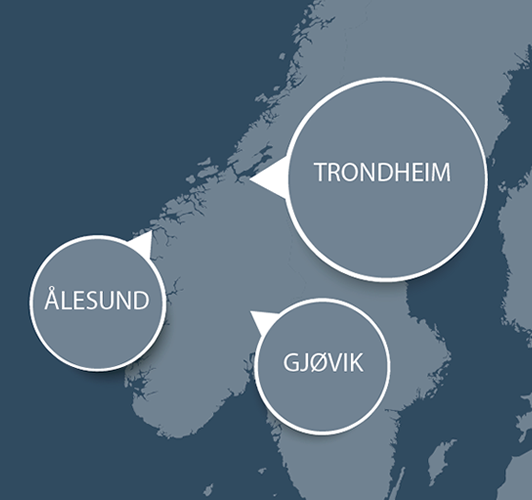
\includegraphics[width=.5\textwidth]{figures/kart_student}
  \caption[Map of NTNU Campuses]{The map shows the three main campuses of NTNU.}
  \label{fig:mapNTNU}
\end{figure}

For figures compsed of several sub-figures, the \texttt{caption} and \texttt{subcaption} packages have been preloaded. See \cref{fig:subfig} with \cref{sfig:a,sfig:b} for an example. For more details on alignment etc., see the Overleaf documentation.\footnote{\url{https://www.overleaf.com/learn/latex/How_to_Write_a_Thesis_in_LaTeX_(Part_3):_Figures,_Subfigures_and_Tables}}

\begin{figure}
    \centering
    \begin{subfigure}[b]{.45\textwidth}
        \centering
        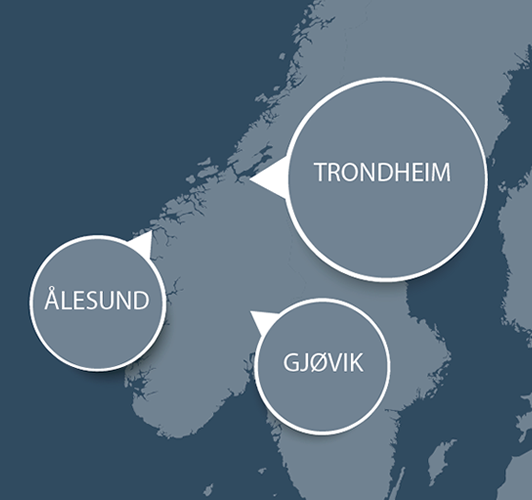
\includegraphics[width=\textwidth]{figures/kart_student.png}
        \caption{First sub-figure}
        \label{sfig:a}
    \end{subfigure}
    \hfill
    \begin{subfigure}[b]{.45\textwidth}
        \centering
        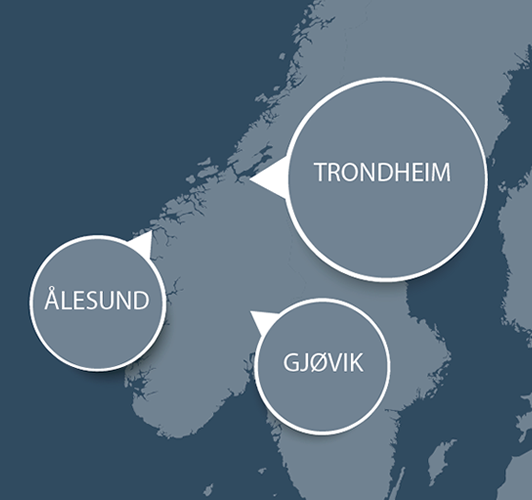
\includegraphics[width=\textwidth]{figures/kart_student.png}
        \caption{Second sub-figure}
        \label{sfig:b}
    \end{subfigure}
    \caption{A figure composed of two sub-figures. It has a long caption in order to demonstrate how that is typeset.}
    \label{fig:subfig}
\end{figure}

You can make nice graphs directly from data files using \texttt{gnuplot}, but it is expensive on every compilation.  The code is included in the
raw latex as a comment so you can uncomment that code to see how it works.
% , for an example, see \cref{fig:examplegnuplot}.
%
%\begin{figure}[htbp]
%  \centering
%    \begin{gnuplot}[terminal=epslatex,terminaloptions={size 8cm,6cm color}]
%        set xlabel "age"
%        set ylabel "IQ"
%        set key autotitle columnhead
%        set title "age vs IQ"
%        set yrange [0:160]
%        set datafile separator ","
%        plot "csvtables/ageiq.csv" using 1:2 with boxes
%    \end{gnuplot}
%  \caption[An example of Integrated Graph]{This is a gnuplot graph read from a file. Also this figure has a long caption in order to demonstrate how that is typeset.}
%  \label{fig:examplegnuplot}
%\end{figure}

\section{Tables}

Tables are placed in the \texttt{table} environment. An example is given in \cref{tab:example1}. Like figures, tables float freely around in the document in accordance with standard \LaTeX{} behaviour. The table caption should be placed \emph{above} the table. If the caption consists of a single sentence fragment (incomplete sentence), it should not be punctuated.

\begin{table}
  \centering
  \caption{A simple, manually formatted example table}
  \label{tab:example1}
  \begin{tabular}{cc}
    \hline
    age  & IQ \\
    \hline
    10   & 110 \\
    20   & 120 \\
    30   & 145 \\
    40   & 120 \\
    50   & 100 \\
    \hline
  \end{tabular}
\end{table}

Tables can also be automatically generated from CSV files using the \texttt{simplecsv} and \texttt{booktab} packages. See \cref{tab:examplecsv} for an example.

\begin{table}[tbp]
  \centering
  \caption[A simple example table generated from a CSV file]{A simple example table generated from a CSV file using \texttt{simplecsv} and \texttt{booktab}}
  \label{tab:examplecsv}
  \csvautobooktabular{csvtables/ageiq.csv}
\end{table}

\section{Listings}

Code listings are included by means of the \texttt{listings} package. Code examples can be read from file or provided inline, and should be given a caption for cross referencing and for appearance in the list of code listings in the thesis frontmatter. If all your code examples are written in the same programming language, you can use, e.g., \texttt{\textbackslash lstset\{language=Python\}} to set the language once and for all. The code is set with the monospace font, and the font size is reduced to allow for code lines up to at least 80 characters without causing line breaks. Options for programming languages, line numbering etc. are provided. Unlike figures and tables, code listings are not floating objects, and will appear at the same position in the typeset document as in the \texttt{.tex} file. If the caption consists of a single sentence fragment (incomplete sentence), it should not be punctuated.

\lstinputlisting[
    caption={Python example from file},
    label=lst:pythonfile,
    language=Python
]{listings/example.py}

\lstinputlisting[%
    caption={C++ example from file},
    label=lst:cppfile,
    language=C++,
    numbers=left
]{listings/example.cc}

\begin{lstlisting}[
    caption={Python code in \LaTeX{} document},
    label=lst:pythondoc,
    language=Python]
import numpy as np
import matplotlib.pyplot as plt

x = np.linspace(0, 1)
y = np.sin(2 * np.pi * x)

plt.plot(x, y)
plt.show()
\end{lstlisting}

\begin{lstlisting}[
    caption={C++ code in \LaTeX{} document},
    label=lst:cppdoc,
    language=C++]
#include <iostream>
using namespace std;

int main()
{
  cout << "Hello, World!" << endl;
  return 0;
}
\end{lstlisting}

\section{Equations}

Equations are typeset as normally in \LaTeX{}. It is common to consider equations part of the surrounding sentences, and include punctuation in the equations accordingly, e.g.,
\begin{equation}
    f(x) = \int_1^x \frac{1}{y}\,dy = \ln x\,.
    \label{eq:logarithm}
\end{equation}
For more advanced symbols like, e.g., $\mathbb{R}, \mathbb{Q}$, the \texttt{amssymb} package is preloaded, and for more advanced mathematical layout the \texttt{amsmath} behaviour is obtained through the \texttt{mathdesign} package. Confer the overleaf documentation for details.\footnote{\url{https://www.overleaf.com/learn/latex/Mathematical_expressions}}

\section{Fonts}

Bitstream Charter at 11pt with the corresponding Mathdesign math fonts have been selected as the main fonts for the thesis template. For code examples, the monospaced font should be used – for this, a scaled version of the DejaVuSansMono to match the main font is preselected. If you would like to use an accompanying sans serif font, the BeraSans has been made available. The standard \LaTeX{} font commands should be used to switch between fonts, e.g.,
\texttt{\textbackslash textit\{\}} \textit{for italics},
\texttt{\textbackslash textbf\{\}} \textbf{for bold face},
\texttt{\textbackslash texttt\{\}} \texttt{for mono spaced}, and
\texttt{\textbackslash textsf\{\}} \textsf{for sans serif}.
For generic \emph{emphasis}, \texttt{\textbackslash emph\{\}} should be applied.

\section{Cross References}
\label{sec:crossref}

For cross references, i.e., references within the document, the \texttt{\textbackslash cref\{\}} command provided byt the \texttt{cleveref} package should be used. Labels are inserted in the document in the standard \LaTeX{} manner. They are case sensitive, so, e.g., a label immediately after a section command refers to that section, while a label within, e.g., a table environment refers to the table. The \texttt{\textbackslash cref\{\}} command also generates the corresponding text. If the document is in English (class options \texttt{british} or \texttt{american}), the cross references are capitalised, whereas if it is in Norwegian (class options \texttt{norsk} or \texttt{nynorsk}), they are not. If you are writing in Norwegian, you should use \texttt{\textbackslash Cref\{\}} at the beginning of a sentence to ensure that the cross reference is correctly capitalised. For examples on usage, see \cref{sec:crossref} in \cref{chap:usage}, \cref{tab:example1}, \cref{fig:mapNTNU}, \cref{eq:logarithm}, \cref{lst:cppfile}, \cref{paper:scrutiny}, and \cref{app:additional}. \Cref{app:additional} at the beginning of a sentence.

The cross references are made into active hyperlinks in the resulting PDF document by the use of the \texttt{hyperref} package. The colour of the links is set to black for best appearance on print. This can easily be changed by the author by the use of the \texttt{\textbackslash hypersetup\{\}} command.

\section{Glossary and Acronyms}
The template comes with the ability to create a glossary and acronym list. To add entries to one of these lists, add them to the \texttt{glossary.tex} file.
All uses of the acronym and glossary functions will create a clickable link that references the corresponding entry in one of the lists. All entries in the lists will also contain page references to all places it has been used.
\subsection{Using Acronyms}
To render acronyms, you have three options:
\begin{itemize}
  \item \texttt{\textbackslash acrlong\{ \}} prints the phrase the acronym stands for, e.g. \texttt{\textbackslash acrlong\{gcd\}} displays \acrlong{gcd}.
  \item \texttt{\textbackslash acrshort\{ \}} prints the acronym, e.g. \texttt{\textbackslash acrshort\{gcd\}} displays \acrshort{gcd}.
  \item \texttt{\textbackslash acrfull\{ \}} prints both the acronym and its definition, e.g. \texttt{\textbackslash acrfull\{gcd\}} displays \acrfull{gcd}.
\end{itemize}

\subsection{Using Glossary}
\begin{itemize}
  \item \texttt{\textbackslash gls\{ \}} prints the term in lowercase, e.g. \texttt{\textbackslash gls\{maths\}} displays \gls{maths}.
  \item \texttt{\textbackslash Gls\{ \}} prints the term in with first letter in uppercase, e.g. \texttt{\textbackslash Gls\{maths\}} displays \Gls{maths}.
  \item \texttt{\textbackslash glspl\{ \}} prints the term in plural form, e.g. \texttt{\textbackslash glspl\{bibliography\}} displays \glspl{bibliography}.
  \item \texttt{\textbackslash Glspl\{ \}} prints the term in plural form capitalized, e.g. \texttt{\textbackslash Glspl\{bibliography\}} displays \Glspl{bibliography}.
\end{itemize}


\section{Bibliography}

The \gls{bibliography} is typset using the \texttt{biblatex} package with the \texttt{biber} backend. The default citation style is \texttt{numeric-comp}, and the default bibliography style is \texttt{numeric}. This produces a bibliography similar to, but not completely according to, the so-called Vancouver style. With this setup, a single \texttt{\textbackslash cite\{\}} command will give a number only~\cite{landes1951scrutiny}, and \texttt{\textbackslash textcite\{\}} will give author and number like this: \textcite{landes1951scrutiny}. If you would like to give the full reference of a paper within the thesis, e.g., in a list of included papers, use \texttt{\textbackslash fullcite\{\}} like this: \fullcite{landes1951scrutiny}.

\section{Included Papers}

If you are writing a compiled PhD thesis (and probably only then – see \cref{sec:compiledphd}), you will need to attach the papers containing the main contribution of the thesis. This can be done issuing the \texttt{paper} environment. It takes two arguments: (i) the PDF file, and (ii) a label for cross referencing. See \cref{paper:scrutiny} for an example.

\section{Appendices}

Additional material that does not fit in the main thesis but may still be relevant to share, e.g., raw data from experiments and surveys, code listings, additional plots, pre-project reports, project agreements, contracts, logs etc., can be put in appendices. Simply issue the command \texttt{\textbackslash appendix} in the main \texttt{.tex} file, and then the following chapters made by \texttt{\textbackslash chapter\{\}} become appendices. See \cref{app:additional} for an example.
